\section{Pixel Processing Unit (PPU)}

{\it WARNING: This section rambles incoherently over a piece of hardware that does not yet exist, marking a complete departure from the preceding documentation}

\begin{figure}[!htb]
\centering
\caption{Pixel processing unit, block-level diagram}
\label{diagram:ppu_block}
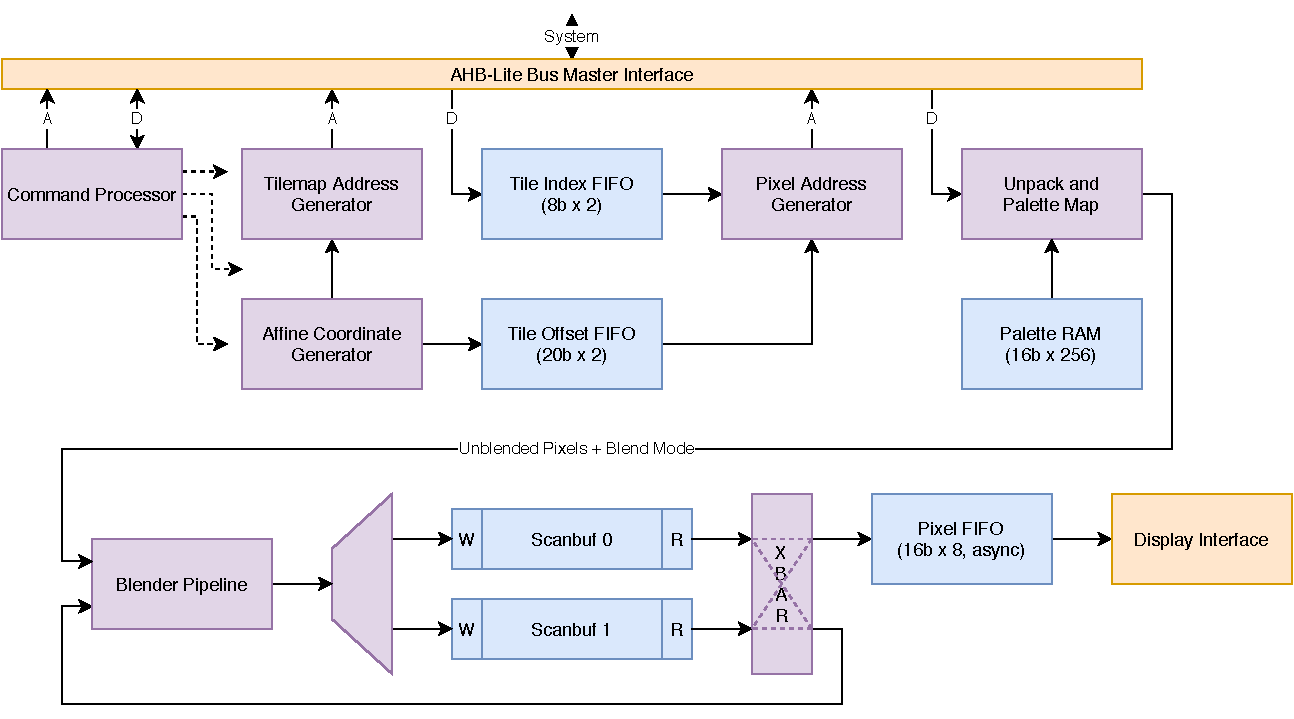
\includegraphics[width=\textwidth]{diagrams/ppu_block.pdf}
\end{figure}

Figure \ref{diagram:ppu_block} shows the high-level structure of the PPU. A number of independent sprite and background engines stream tile and pixel data from system memory, each producing a pixel stream which is continous in the case of the backgrounds, and generally sparse in the case of sprites. These multiple streams are blended according to transparency and layer order. Finally, any paletted pixels are looked up in the shared palette RAM, to produce full-colour pixels for the display.

The PPU makes no assumptions about display timing: for example, RISCBoy is currently equipped with a 320$\times$240 SPI LCD, which is driven continuously, with no horizontal or vertical blanking periods, as the SPI interface is the framerate bottleneck. The PPU continuously generates pixels at some rate which is hopefully higher than the display scan rate, and its timing is decoupled from the display via the pixel FIFO (as this is the narrowest point of the PPU, so the cheapest to buffer).

A key feature is the Poker: this is a simple raster-synchronised coprocessor that allows the PPU to modify its own configuration with pixel-perfect timing, enabling advanced rendering tricks such as in-scanline sprite multiplexing.

\subsection{Pixel Formats}

Internally, the PPU uses a single native pixel format, namely ARGB 1555 (see figure \ref{diagram:pixformat}), but to save bandwidth, the PPU can stream pixels from memory in a variety of formats, and convert internally. These range down to 1 bit per pixel, for both sprites and tiles. PPU memory accesses are \textbf{always little-endian}: for performance reasons the PPU performs the widest possible fetch, yielding multiple pixels each, which are numbered least-significant-first.

\begin{figure}[!htb]
\centering
\caption{PPU pixel formats}
\label{diagram:pixformat}
\begin{tabular}{r l}
	\raisebox{-1ex}[5ex][1.5ex]{
		\begin{bytefield}[endianness=big,bitformatting=\small, bitwidth=auto]{16}
		\bitheader{0,4,5,9,10,14,15} \\
		\bitbox{1}{A} \bitbox{5}{R} \bitbox{5}{G} \bitbox{5}{B}
		\end{bytefield}} & ARGB 1555, alpha = 0 when transparent \\
		\\
	\raisebox{-1ex}[5ex][1.5ex]{
		\begin{bytefield}[endianness=big,bitformatting=\small, bitwidth=auto]{16}
		\bitheader{0,4,5,9,10,14,15} \\
		\bitbox{1}{} \bitbox{5}{R} \bitbox{5}{G} \bitbox{5}{B}
		\end{bytefield}} & RGB 555, alpha bit is ignored (always opaque) \\
		\\
	\raisebox{-1ex}[5ex][1.5ex]{
		\begin{bytefield}[endianness=big,bitformatting=\small, bitwidth=auto]{8}
		\bitheader{0,1,2,4,5,6,7} \\
		\bitbox{1}{A} \bitbox{2}{R} \bitbox{3}{G} \bitbox{2}{B}
		\end{bytefield}} & ARGB 1232, alpha = 0 when transparent \\
		\\
	\raisebox{-1ex}[5ex][1.5ex]{
		\begin{bytefield}[endianness=big,bitformatting=\small, bitwidth=auto]{8}
		\bitheader{0,1,2,4,5,6,7} \\
		\bitbox{1}{} \bitbox{2}{R} \bitbox{3}{G} \bitbox{2}{B}
		\end{bytefield}} & RGB 232, alpha bit is ignored (always opaque) \\
		\\
	\raisebox{-1ex}[5ex][1.5ex]{
		\begin{bytefield}[endianness=big,bitformatting=\small, bitwidth=auto]{8}
		\bitheader{0,7} \\
		\bitbox{8}{Index}
		\end{bytefield}} & P8: an index into a table of 256 colours\\
		\\
	\raisebox{-1ex}[5ex][1.5ex]{
		\begin{bytefield}[endianness=big,bitformatting=\small, bitwidth=auto]{4}
		\bitheader{0,3} \\
		\bitbox{4}{Index}
		\end{bytefield}} & P4: an index into a table of 16 colours \\
		\\
	\raisebox{-1ex}[5ex][1.5ex]{
		\begin{bytefield}[endianness=big,bitformatting=\small, bitwidth=auto]{2}
		\bitheader{0,1} \\
		\bitbox{2}{Idx}
		\end{bytefield}} & P2: an index into a table of 4 colours \\
		\\
	\raisebox{-1ex}[5ex][1.5ex]{
		\begin{bytefield}[endianness=big,bitformatting=\small, bitwidth=auto]{1}
		\bitheader{0} \\
		\bitbox{1}{I}
		\end{bytefield}} & P1: an index into a table of 2 colours \\
		\\
\end{tabular}
\end{figure}

Background pixel format is configured per-background; sprite pixel format is configured globally.

For pixels smaller than one byte, the pixel order continues to be defined in a little-endian fashion, i.e. the least-significant pixel will be the first to be displayed. There is an additional constraint that all pixels be naturally aligned in memory. That is, pixel address modulo pixel size is zero.

A paletted pixel is transparent if:

\begin{itemize}
	\item The colour index is 0, and
	\item Transparency is enabled for that pixel source
\end{itemize}

So at e.g. 1 bit per pixel, it is possible to have either 2 colours, or 1 colour plus transparency. It is important that the transparency of a pixel is known as early as possible: this enables the PPU to perform layer composition before palette lookup, so only one palette lookup per {\it screen} pixel is required.


\subsection{Palettes}

The PPU contains a single hardware palette memory (PRAM). The PRAM is large enough to store 256 colours in RGB 555 format. Each pixel in a paletted image (see figure \ref{diagram:pixformat}) consists of an index into PRAM. The PPU looks these indices up before passing pixels to the screen; wide colour range is maintained at reduced bits per pixel.

Although there is only a single hardware palette, 256 colours in size, backgrounds and sprites can index this palette at an offset. PRAM may be initialised with e.g. multiple 16-colour tables at different (potentially overlapping) locations, giving effectively independent palettes.

PRAM can be addressed through the PPU's configuration interface, for configuration by the system. The PPU has priority access to the PRAM, so attempting to access PRAM during drawing may cause a lengthy stall. As with all PPU configuration state, it can also be updated by the Poker, using a {\tt poke} instruction; under ideal conditions the PPU can completely replace PRAM contents in 257 cycles.

\subsection{Layers}

Each background, and each sprite, can be individually assigned a layer number in the range $0 \leq n < N$, where $N$ is the layer count (configurable). The number of layers is wholly independent from the number of sprites, backgrounds, etc., and may be as little as 1. For each blended pixel, the blender observes non-transparent pixels from each source (sprite or background), and applies the following rules:

\begin{itemize}
	\item If there are no input pixels, output the display background colour.
	\item Else output the pixel with the lowest layer number
	\item If there are multiple pixels on the same layer:
	\begin{itemize}
		\item Sprites beat backgrounds
		\item Lower-numbered sprites beat higher-numbered
		\item Lower-numbered backgrounds beat higher-numbered
	\end{itemize}
\end{itemize}

Layer number can be thought of as depth into the screen. X is positive to the right, and Y is positive downward, so in a right-handed coordinate system, Z would be positive into the screen.

\subsection{Backgrounds}

Backgrounds are composed of tiles. Tiles are composed of pixels.

\begin{figure}[H]
\centering
\caption{PPU background coordinate system}
\label{diagram:ppu_bg_coords}
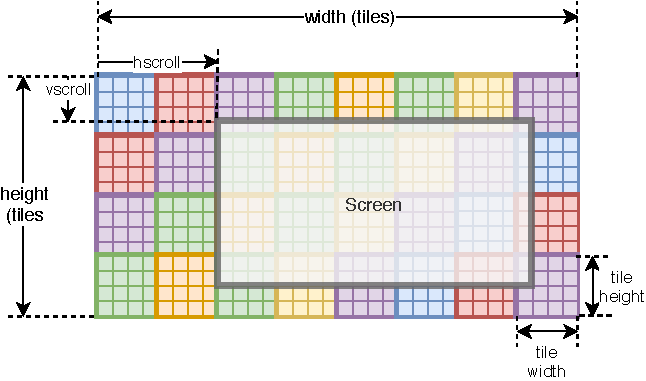
\includegraphics[width=0.7\textwidth]{diagrams/ppu_bg_coords.pdf}
\end{figure}

Each tile is a square image, the width and height of which (measured in pixels) is configured per-background, and is always a power of two. Tiles are stored as part of a larger image, known as the tileset. Tiles are numbered in a row-major order, starting at the top left of the tileset. An example tileset is shown in figure \ref{diagram:ppu_tileset}: this is a tileset of 8 tiles, each $4\times 4$ pixels in size.

\begin{figure}[H]
\centering
\caption{Example PPU tileset}
\label{diagram:ppu_tileset}
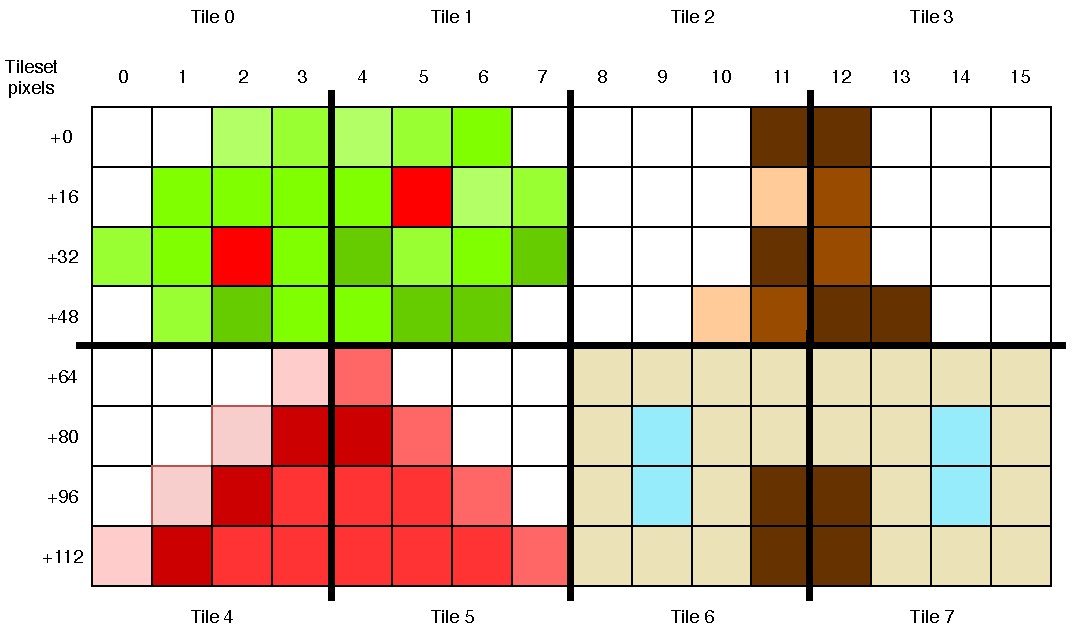
\includegraphics[width=0.7\textwidth]{diagrams/ppu_tileset.pdf}
\end{figure}

Each pixel row of the tileset is stored as a packed array of pixels in memory, and the next row follows. Note that all tiles must be the same size, and have the same pixel format.

The complete background image is assembled from these tiles. The arrangement is specified the tilemap: a grid of numbers, each naming a tile from the tileset. For each pixel on the screen, the tilemap tells the PPU which tile should be at that location, and the corresponding tile image in the tileset tells the PPU the colour of each pixel in that screen tile. This is shown in figure \ref{diagram:ppu_tilemap}.

\begin{figure}[H]
\centering
\caption{Example PPU tilemap}
\label{diagram:ppu_tilemap}
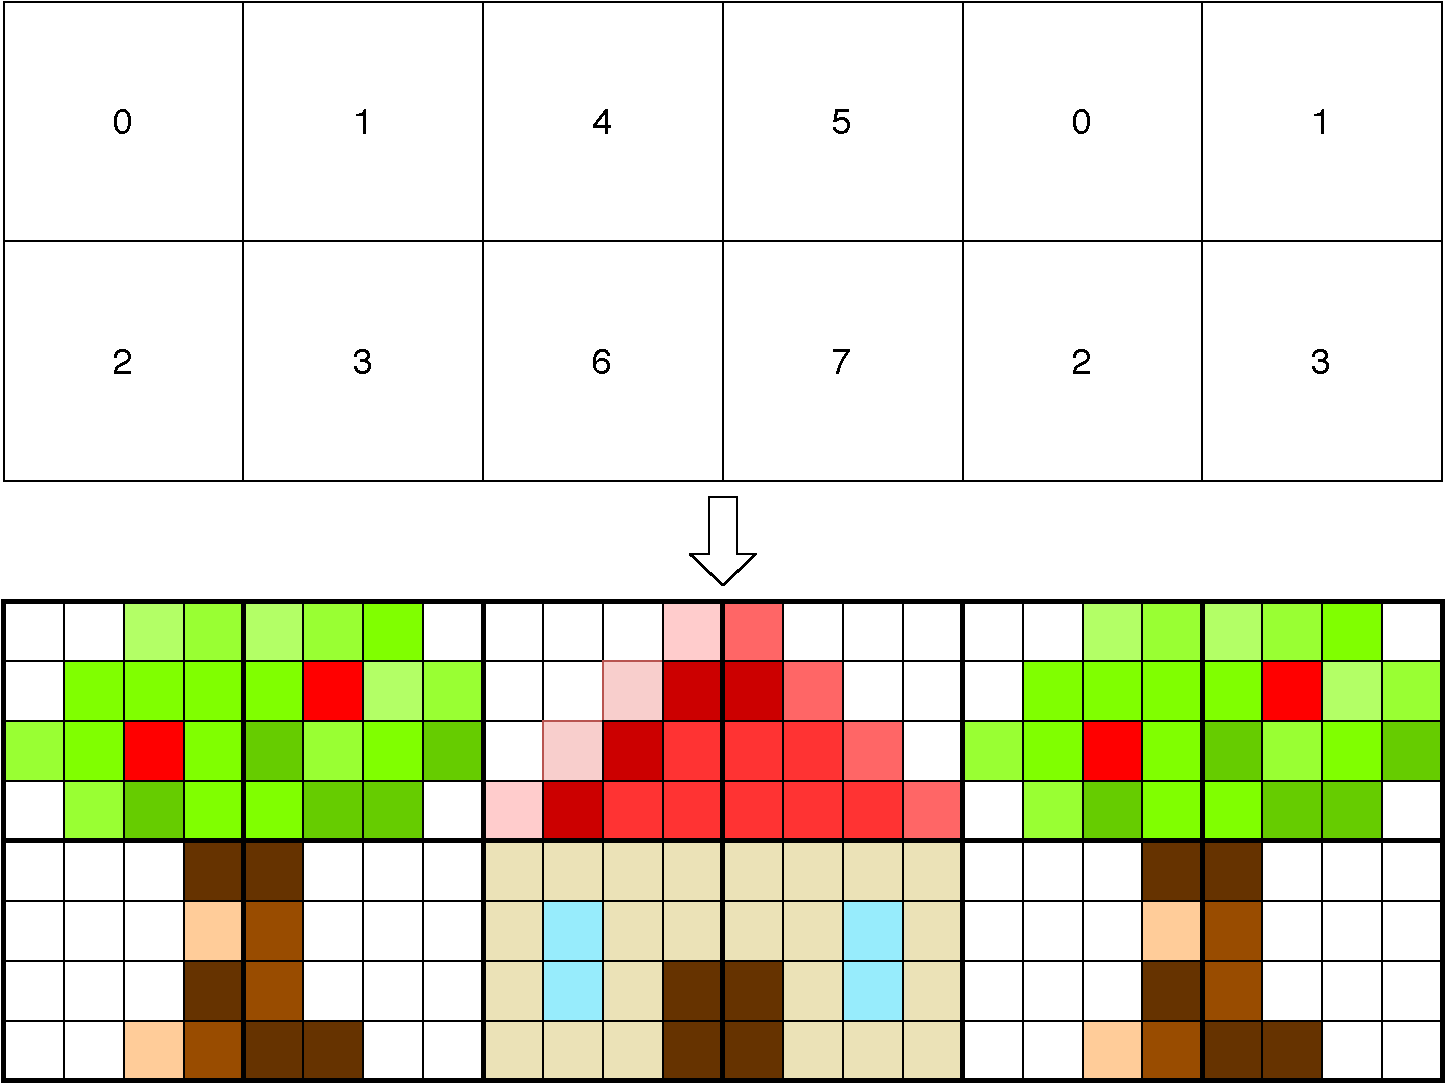
\includegraphics[width=0.7\textwidth]{diagrams/ppu_tilemap.pdf}
\end{figure}

The screen origin is offset into the background by configuring the horizontal and vertical scroll. This allows the game view to move smoothly over a fixed background. If the screen area overhangs the background, coordinates are wrapped.

In total, a background is defined by:

\begin{itemize}
	\item Width and height, measured in pixels
	\item Horizontal and vertical scroll, measured in pixels
	\item Tileset:
	\begin{itemize}
		\item Tile pixel format
		\item Tile size in pixels (power of two)
		\item Tileset width in pixels (power of two)
		\item Pointer to the tileset image (aligned to row size in bytes)
	\end{itemize}
	\item Tilemap:
	\begin{itemize}
		\item Pointer to the tilemap buffer
	\end{itemize}
\end{itemize}

This tilemapping process allows detailed images to be displayed with a minimal memory footprint, compared with a framebuffer, which must store the colour of every single pixel on the screen. Backgrounds can also be configured to not perform tilemapping, and simply scan out the entire tileset image to the screen (this is the same as assuming the tilemap is $[0, 1, 2, 3, 4....]$), so the tileset can be used as a framebuffer. Software can then render graphics directly to this framebuffer, and the PPU will simply display it as a background layer.

\subsection{Sprites}

Sprites are small images which can be displayed at arbitrary screen coordinates; for example, the player character.

\subsection{Pixel Gearboxes}

One design challenge the PPU faces is the high ratio of data bus width to smallest pixel size (32:1). Another is the wide variety of pixel sizes (16 $\to$ 1 bits). Consequently, to make efficient use of the bus, sprite and tile engines must be able to capture the result of one bus read, and parcel it out over a number of clock cycles.

A naive but effective implementation is a databus-sized register with mux taps to perform shift-by-16, shift-by-8, and so on, for each pixel size. Unfortunately, this is much too large -- around 120 LUTs on iCE40, if you include the extra mux for loading bus data. Savings can be made by noting we can trash data which will not reach the end (e.g. no need to zero the top half on a shift-by-16), but it is not enough for a component which will be in every sprite and tile engine. The number of taps could be reduced, but this carries a performance cost.

To improve on this, the key observation is that the total shift count will always be 0, modulo the pixel size. Put differently, every shift starts on a bit boundary aligned to at least the size of that shift.

The hardware scheme used by the pixel gearbox is:
\begin{itemize}
	\item There is a register the same size as the databus.
	\item The left half of this register can be copied to the right half
	\item This continues recursively, to the right:
	\begin{itemize}
		\item The left half of the right half can instead be copied to the right half of the right half
		\item The left half of {\it this} can instead be copied to the right half of this
		\item So on, down to one bit
	\end{itemize}
\end{itemize}

This is dramatically smaller, because the number of mux taps is exponentially distributed over the bits: half of the flops have no taps, a quarter have one, an eighth have two, and so on. (Ignoring the tap used for loading all flops from data bus.) On iCE40 this is 40 LUTs per gearbox, for a 32 bit databus and 1 bit minimum pixels.

\begin{figure}[H]
\centering
\caption{Pixel gearbox, shift-by-8}
\label{diagram:pixel_gearbox_8}
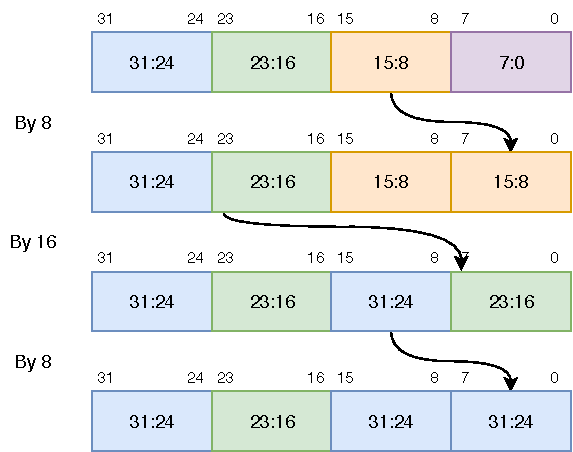
\includegraphics[width=0.5\textwidth]{diagrams/pixel_gearbox_8.pdf}
\end{figure}

Figure \ref{diagram:pixel_gearbox_8} shows the sequence for shifting 8-bit pixels through the pixel gearbox. Note that the time-ordered sequence of pixels down the rightmost column is the same as the right-to-left sequence in the top row (recall pixel order is little-endian). All of the shift sizes are possible; proof is left as an exercise!

Based on the above observation about naturally-aligned boundaries, there is a very satisfying way of generating the control signals for the gearbox:

\begin{itemize}
	\item Initialise a counter
	\item Every clock, the counter increments by the shift amount
	\item The next counter value will always have exactly one bit set which is not set in the current counter value (this is a property of counters)
	\item The weight of this bit is equal to the copy stride of the gearbox for this cycle
\end{itemize}

I.e. \verb|shamt = ctr_next & ~ctr|. In figure \ref{diagram:pixel_gearbox_8} the counter values would be 0b00000, 0b01000, 0b10000, 0b11000, hence the strides are 8, 16, 8.

Note that this control scheme also allows rapid (log-time) seeking to arbitrary offsets, by adding first the MSB of the offset to the counter, then the next bit, and so on. This maintains the invariant that we are aligned to a shift-sized boundary, since we have sorted our shifts in descending size order.

\subsection{Poker}
\label{section:ppu_poker}

The Poker is a programmable component of the PPU, inspired by the Amiga Copper. It allows the PPU to manipulate its own controls, with pixel-perfect timing. There are no restrictions on when this takes place, or what is changed.

This enables acrobatic feats such as multiplexing a single sprite back-to-back down a scanline. However, Poker execution does have a performance cost, as Poker instructions are fetched through the same memory interface as pixel data. Reconfiguring some pieces of hardware (e.g. a background engine) mid-scanline may trigger flushing of that hardware, which is also wasteful. Overuse may cause missed pixels.

Poker instructions reside in main system memory. Instructions are documented below. The instruction set is designed to be simple to decode and simple to generate dynamically, not to have high code density!

\subsubsection*{WAIT}

\begin{bytefield}[endianness=big,bitformatting=\tiny]{32}
\bitheader{0,11,12,23,24,31} \\
\bitbox{8}{{\tt WAIT}} \bitbox{12}{{\tt x}} \bitbox{12}{{\tt y}} \\
\end{bytefield}

Suspend execution, resuming immediately before pixel ({\tt x}, {\tt y}). For example {\tt WAIT 0, 0} will halt Poker execution until the start of the next frame. The Poker should generally spend most of its time in a suspended state, as it blocks pixel data fetches while it is executing.

Setting {\tt x} or {\tt y} to the all-ones bit pattern means "any". For example, the Poker may scan a block of sprite configuration at the start of every line, or change background colour at a certain point on every scanline.

Any pixels before ({\tt x}, {\tt y}) are unaffected by any changes the Poker may make. Once the Poker finishes poking, and goes back into the {\tt WAIT} state, all pixels after this point (inclusive of ({\tt x}, {\tt y}) take the new values into account.

\subsubsection*{POKE}

\begin{bytefield}[endianness=big,bitformatting=\tiny]{32}
\bitheader{0,15,24,31} \\
\bitbox{8}{{\tt POKE}} \bitbox{8}{{\tt count}} \bitbox{16}{{\tt addr}} \\
\bitheader{0, 31} \\
\bitbox{32}{{\tt data}} \\
\end{bytefield}

Write {\tt data} into the PPU's configuration address space, starting at {\tt addr}. The {\tt data} payload is ${\tt count}+ 1$ words in size. Absolutely any state can be modified, but beware that each pixel engine (sprite or background) will perform a reload when relevant config is written to.

For example, a background may have its tileset {\tt POKE}d at a certain point in each scanline, if there is a menu on the side of the screen which uses a font tilemap to draw text.

Some {\tt POKE}s are more expensive than others: it is possible to change the vertical scroll for every single pixel along a scanline, and this will produce the expected image. However, scrolling the screen invalidates the state of all sprites and backgrounds, which may cause slowdown if done too often.

Note that the Poker's program counter is mapped into the configuration address space; {\tt POKE} can be used to perform jumps.

\subsubsection*{SPRITE}

\begin{bytefield}[endianness=big,bitformatting=\tiny]{32}
\bitheader{0,7,8,15,16,23,24,31} \\
\bitbox{8}{{\tt SPRITE}} \bitbox{8}{count} \bitbox{8}{{\tt start}} \bitbox{8}{{\tt end}} \\
\bitheader{0, 31} \\
\bitbox{32}{{\tt addr}} \\
\end{bytefield}

Scan through {\tt count} sprite configuration words starting at {\tt addr} and assign them to sprites in range {\tt start}...{\tt end} if they intersect the current scanline. Disable remaining sprites. Stop scanning if {\tt end} is reached. If the display has a horizontal blanking period, this is the ideal time to perform {\tt SPRITE} scanning. This instruction is implemented with hardware already present in the PPU, so presents little extra cost.

This mechanism is similar to GameBoy OAM search. The effect is that the user can define a large number of virtual sprites -- more than are available in hardware -- and the PPU can draw all of these, as long as the number of sprites on one scanline is not greater than the hardware sprite count.

Alternatively, sprite allocation can be performed by software, and the sprites updated using a {\tt POKE} instruction. The {\tt POKE} approach is more flexible, and makes it easier to multiplex hard sprites within a single scanline.

\subsubsection*{SKIP}

\begin{bytefield}[endianness=big,bitformatting=\tiny]{32}
\bitheader{24,31} \\
\bitbox{8}{{\tt SKIP}} \bitbox{24}{TBD} \\
\end{bytefield}

Skip the following instruction, if the beam has reached some point. Full details TBD. It might be better to provide a conditional jump with a target, because not all of our instructions are the same length (especially {\tt POKE})

This allows Poker loops to be programmed, and makes the wait wildcard values much more useful.
